\documentclass[12pt]{article}
\usepackage{latexsym}
\usepackage{amssymb,amsmath}
\usepackage[pdftex]{graphicx}
\usepackage{epstopdf}


\topmargin = 0.1in \textwidth=5.7in \textheight=8.6in

\oddsidemargin = 0.2in \evensidemargin = 0.2in


\begin{document}

\begin{center}
COMPUTER SCIENCE 20, SPRING 2014 \\
Homework Problems\\
Recursive Definitions, Structural Induction, States and Invariants\\
Author: Tawheed Abdul-Raheem
\end{center}

\smallskip

\subparagraph*{Note:}
Use the following definition of the set of valid integer binary trees $T$.
\begin{itemize}
\item \textbf{Base Cases:} $$\epsilon \in T$$
\item \textbf{Constructor Case:} If $x \in \mathbb{Z}$, $l \in T$, $r \in T$, then
$$(x,l,r) \in T$$
\item A \textit{node} of a tree is any element in $T$ that is a three-tuple, that is, it is of the form $(x,l,r)$. This means that $\epsilon \in T$ is not a node.
\item If $z = (x,l,r)$ is a node, then $l$ and $r$ are child nodes of $z$, if they are non-empty.
\end{itemize}
\begin{enumerate}
\item The nodes in a tree obey the \textit{heap property} if, for every node $z$ in the tree, the value in $z$, that is $x$, is at least as big as the value in each of $z$'s children (the tree in module 15 obeys the heap property).\\\\
Prove that if a binary tree has the heap property, then the value in the root of the tree is at least as large as the value in any node of the tree.
\item A \textit{complete} binary tree (example below) is a binary tree in which every level, except possibly the last level, is completely filled, and all nodes are as far left as possible.
\begin{center}
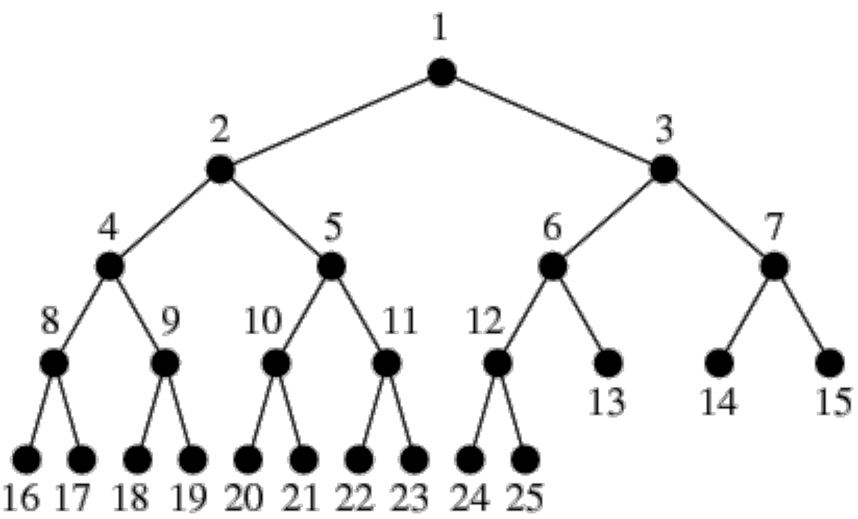
\includegraphics[scale=.3]{CompleteBinaryTree.pdf}
\end{center}
Also, remember that an \textit{internal node} is a node that has children.\\\\
Prove that the number of internal nodes in a complete binary tree with $n$ nodes is $\lfloor n/2 \rfloor$ where $\lfloor x \rfloor$ equals the largest integer that is not greater than $x$.
\item (From Meyer, problem 6.6) Let $m,n \in \mathbb{Z}$ where $m \not = 0$ and $n \not = 0$. Then, let's define a set of integers, $L_{m,n}$, recursively as follows:
\begin{itemize}
\item \textbf{Base cases:} $m,n \in L_{m,n}$
\item \textbf{Constructor cases:} If $j,k \in L_{m,n}$, then
\begin{enumerate}
\item $-j \in L_{m,n}$. and
\item $j + k \in L_{m,n}$
\end{enumerate}
\end{itemize}
Let $L$ be an abbreviation for $L_{m,n}$ for the rest of this problem.
\begin{enumerate}
\item Prove by structural induction that every common divisor of $m$ and $n$ also divides every member of $L$.
\item Prove that any integer multiple of an element of $L$ is also in $L$.
\item Show that if $j,k \in L$ and $k \not = 0$ then the remainder of $j$ divided by $k$ is also in $L$; that is, that  $\mathsf{rem}(j,k) \in L$.
\end{enumerate}
\item (From Sipser, exercise 1.6) Draw state machines that only accept strings in the following set. Assume that the alphabet is $\Sigma = \{0,1\}$; that is, that all strings $s \in \Sigma^*$.\\ (Bonus point(s) if you draw your raw state machines in LaTeX; check out the TikZ package to do this.)
$$\{w:w \text{ contains the substring 0101, i.e. }w = x0101y \text{ for some }x \text{ and }y\}$$
\item (From Meyer, problem 5.29) A robot named Wall-E wanders around a two-dimensional grid. He starts at (0,0) and is allowed to take four different types of steps:
\begin{enumerate}
\item (+2,-1)
\item (+1, -2)
\item (+1, +1)
\item (-3, 0)
\end{enumerate}
For example, Wall-E might take the following stroll. The types of his steps are denoted by each arrow's subscript:
$$(0,0) \to^a (2,-1) \to^c (3,0) \to^b (4,-2) \to^d (1,-2) \to \ldots$$
Wall-E's true love, the fashionable and high-powered robot, Eve, awaits at (0,2).
\begin{enumerate}
\item Describe a state machine model of this problem.
\item Will Wall-E ever find his true love? Either find a path from Wall-E to Eve or use the Invariant Principle to prove that no such path exists.
\end{enumerate}
\end{enumerate}



\end{document}
